\section{Exercises}
\label{section:sequentialCircuitsExercises}
\graphicspath{ {./chapter05/FigHw} }

\begin{enumerate}

\item \textbf{ (8 pts.)}Determine the state table for the circuit in Figure~\ref{fig:sequentialCirNANDs}.
\begin{figure}[ht]
\center{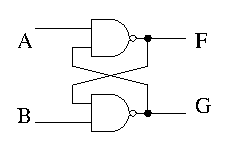
\includegraphics{Prob5-1}}
\caption{}
\label{fig:sequentialCirNANDs}
\end{figure}


\begin{onlysolution}  \textbf{Solution} \itshape{
The analysis of the cross-coupled NANDs show in Figure~\ref{fig:sequentialCirnand} is
almost exactly the same as that for the cross coupled NORs.  Start with
the truth table for an NAND gate:

\begin{tabular}{l|l||l}
a & b & (ab)' \\ \hline
0 & 0 & 1 \\ \hline
0 & 1 & 1 \\ \hline
1 & 0 & 1 \\ \hline
1 & 1 & 0 \\ 
\end{tabular}

Observe that the output is 1 whenever
either input is 0.  Now onto the state table for the cross coupled NANDs:

\begin{tabular}{l|l||l|l}
A & B & $F^+$ & $G^+$ \\ \hline
0 & 0 & 1 & 1 \\ \hline
0 & 1 & 1 & 0 \\ \hline
1 & 0 & 0 & 1 \\ \hline
1 & 1 & F & G \\ 
\end{tabular}

For the cross coupled NANDs the output holds when the input $A,B=1,1$ occurs.
In fact if you compare this table to that of the cross coupled NORs, you will
notice that $A,B = S',R'$ and $F,G = Q,Q'$.
} \end{onlysolution} 

\item \textbf{ (8 pts.)} Determine the state table for the circuit 
in Figure~\ref{fig:sequentialCirDLatch}.  Which basic memory element does it act 
like?  Hint, one of the inputs is acting like a clock.  Additional
hint, in order to simplify the analysis, replace a portion of the 
circuit with a component from this chapter.
\begin{figure}[ht]
\center{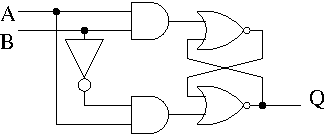
\includegraphics{Prob5-2}}
\caption{}
\label{fig:sequentialCirDLatch}
\end{figure}

\begin{onlysolution}  \textbf{Solution} \itshape{
The main idea in this problem is to simplify the cross coupled NOR gates into
an SR latch.  Then use the state table for the SR latch.  This substitution
will simplify the analysis of this circuit.  Since the lower NOR gate is denoted
$A$, call the lower input of the SR latch $R$ and the upper input $S$
(see Figure 5.6).

This yields the following truth table:

\begin{tabular}{l|l|l|l|l||l}
A & B & S & R & comment & $Q^+$ \\ \hline
0 & 0 & 0 & 0 & Hold    & $Q$   \\ \hline
0 & 1 & 0 & 0 & Hold    & $Q$   \\ \hline
1 & 0 & 0 & 1 & Reset   & 0     \\ \hline
1 & 1 & 1 & 0 & Set     & 1     \\ 
\end{tabular}

It is behaving exactly like a D clocked latch, where $A=clk$ and $B=D$.
} \end{onlysolution} 

\item \textbf{ (8 pts.)} Complete the timing diagram for the circuit 
shown in Figure~\ref{fig:sequentialCirDMS}.  Which basic memory element 
does this circuit act like? 

\begin{figure}[ht]
\label{fig:sequentialCirnand}
\center{\scalebox{0.8}{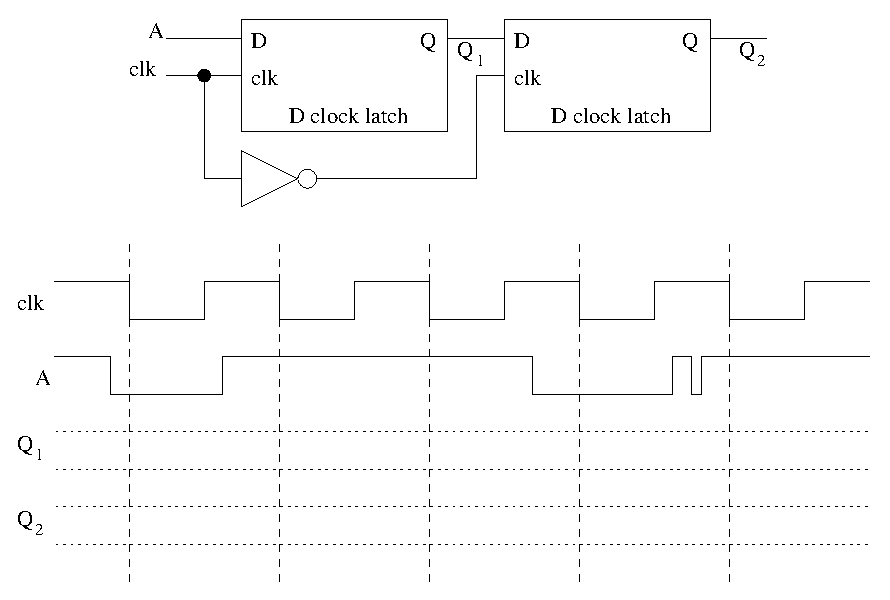
\includegraphics{Prob5-3}}}
\caption{A 2-stage sequential circuit.}
\label{fig:sequentialCirDMS}
\end{figure}

\item \textbf{ (15 pts.)} Complete the timing diagram for the basic memory 
elements in Figure~\ref{fig:sequentialCirExTim}.  The clock cycle is 20 ns. When 
necessary, assume that $Q$ is initialized to 0 and the output settles to 
0 after a period of rapid toggling. 

\begin{figure}[ht]
\center{\scalebox{0.5}{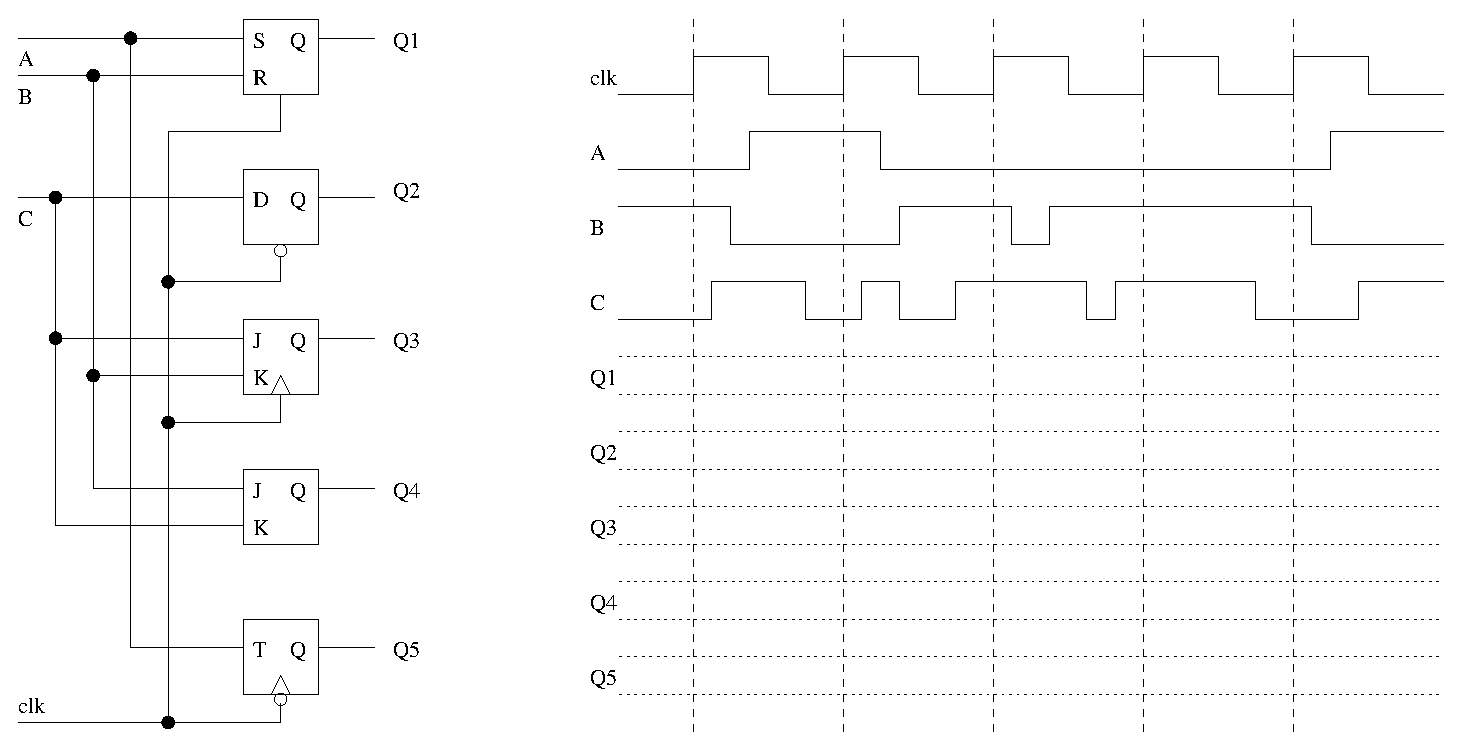
\includegraphics{Prob5-4}}}
\caption{A variety of basic memory elements and the signals applied to them.}
\label{fig:sequentialCirExTim}
\end{figure}

\begin{onlysolution}  \textbf{Solution} \itshape{
\begin{figure}[ht]
\center{\scalebox{0.5}{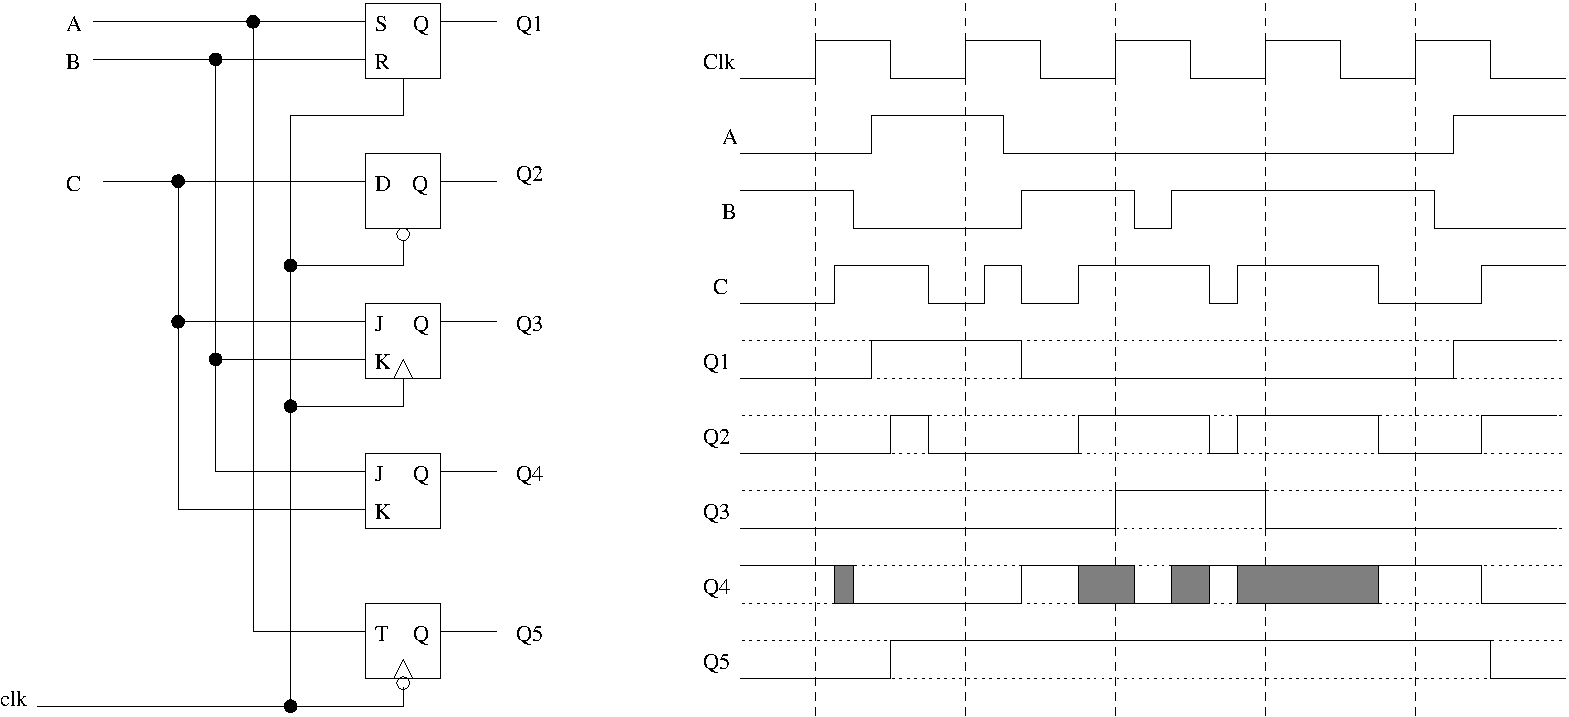
\includegraphics{Sol5-4}}}
\end{figure}
} \end{onlysolution} 


\item \textbf{ (15 pts.)} Complete the timing diagram for the basic memory elements in 
Figure~\ref{fig:sequentialCirExTim2}.  The clock cycle is 20 ns. When necessary, 
assume that Q is initialized to 0 and the output settles to 0 after 
a period of rapid toggling. 
\begin{figure}[ht]
\center{\scalebox{0.5}{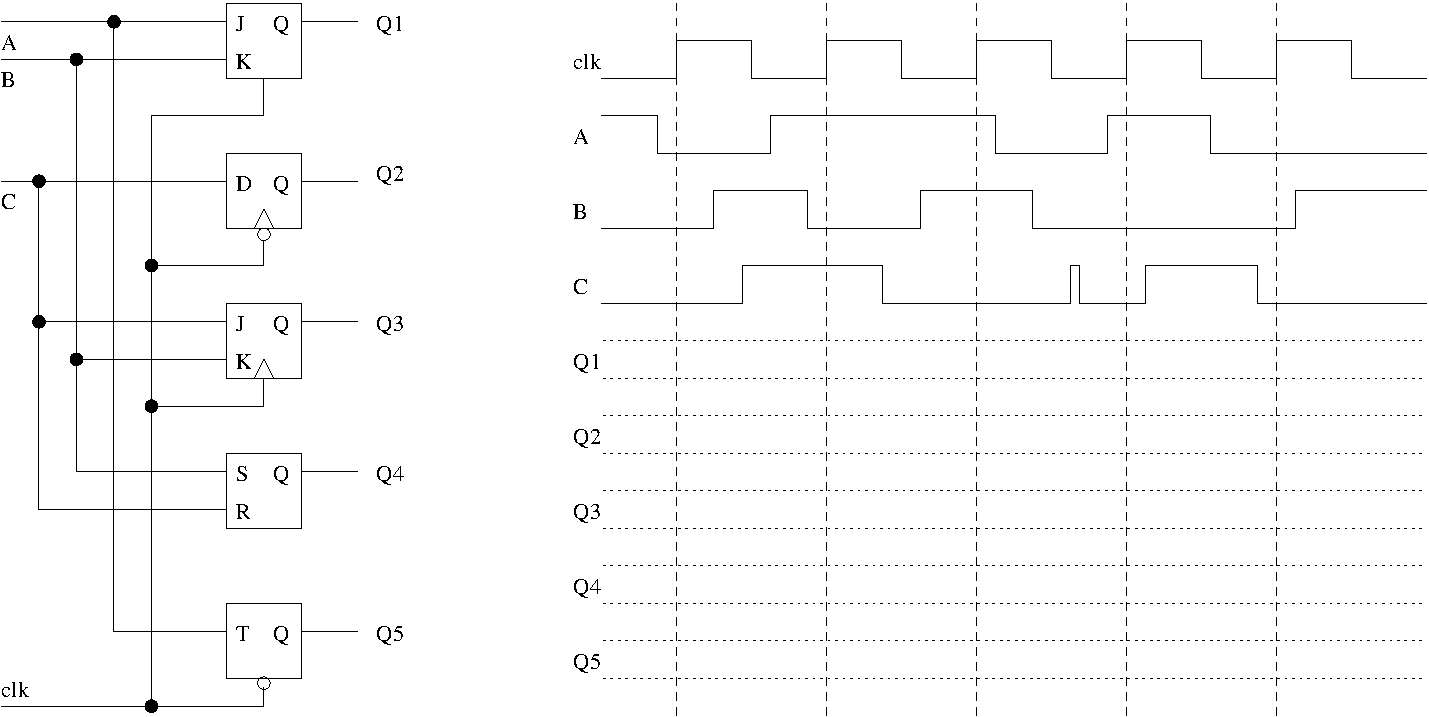
\includegraphics{Prob5-5}}}
\caption{}
\label{fig:sequentialCirExTim2}
\end{figure}

\begin{onlysolution}  \textbf{Solution} \itshape{
\begin{figure}[ht]
\center{\scalebox{0.5}{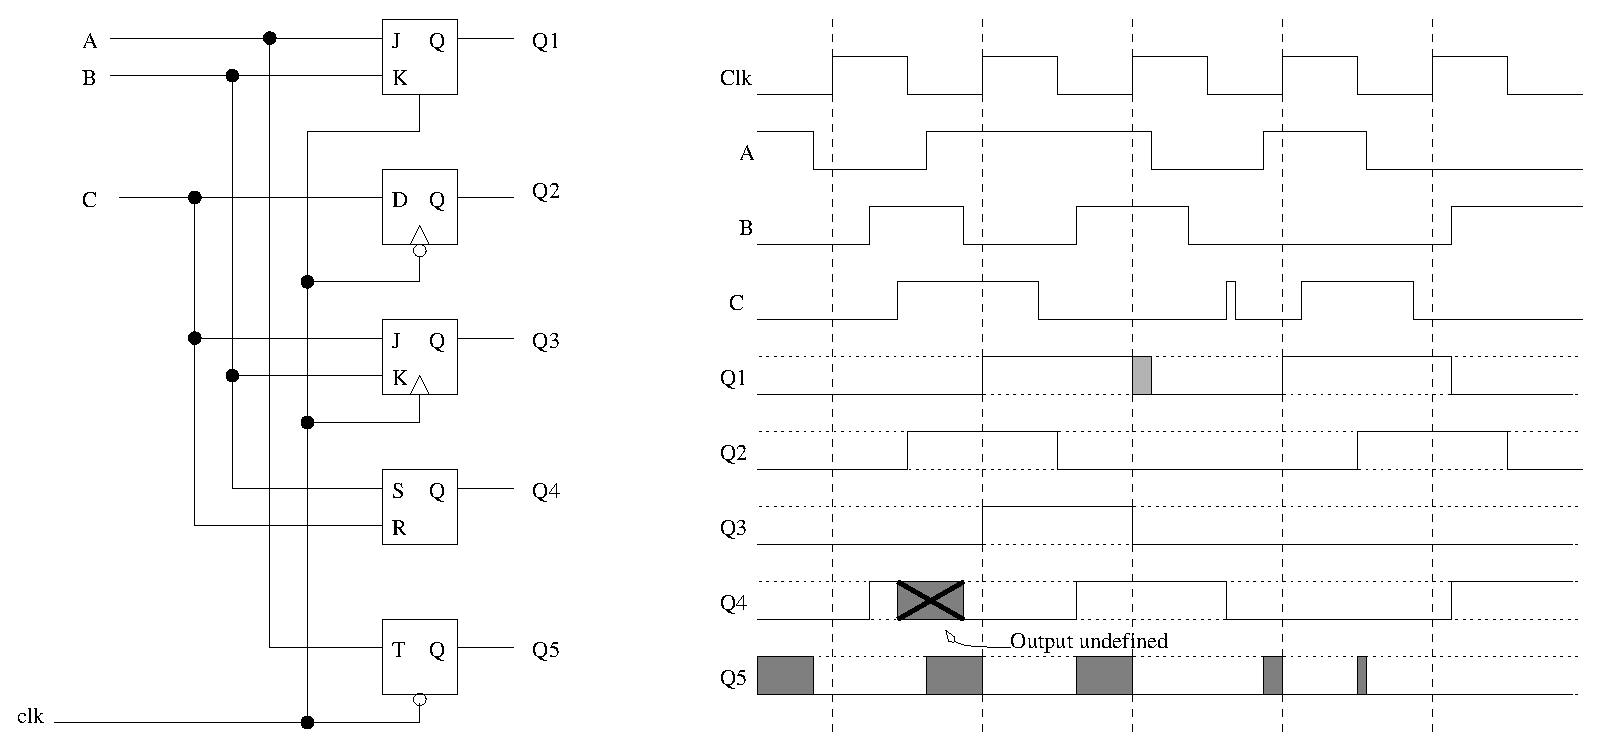
\includegraphics{Sol5-5}}}
\end{figure}
} \end{onlysolution} 


\item \textbf{ (4 pts.)} Consider the furnace 
controller discussed at the beginning of this chapter.  Determine 
which state the controller should transition into when in a particular state
and given a particular combination of inputs.  
Fill in the eight entries in the following table with the next state
the system should move into.  The next state should be either ON if the 
system should transition (or remain in) the ON state, OFF if the system 
should transition (or remain in) the OFF state, or X if the input 
combination is meaningless. 

\begin{table}[ht]
\center{
\begin{tabular}{c||c|c|c|c}
Current State $\bs T_{hi} T_{low}$& 00	& 01	& 11	& 10	\\ \hline \hline
	ON			&	&	&	&	\\ \hline
	OFF			&	&	&	&	\\ 
\end{tabular}
}
\end{table}
 
\item \textbf{ (8 pts.)} Derive the next state equations for each 
type (D, T, SR, and JK) of basic memory element.  The next state equation 
is a symbolic equation describing the next state ($Q^+$) 
as a function of the inputs (D,T,SR, or JK) and state ($Q$).
In order to determine the next state equations for a
a JK memory element, build a 3-variable Kmap with 
$Q$, $J$, and $K$ as the inputs.  The entries in the Kmap should 
be $Q^+$.  Solving this Kmap will yield the next state equation.
Show all work for full credit.

\item \textbf{ (16 pts.)} Derive the transition list for each
type (D, T, JK, and SR) of basic memory element.  A transition 
list describes the input(s) necessary to elicit a particular 
change in state.  For example, imagine that a D flip flop output
is currently in the 0 state and it needs to transition to 
the 1 state after the clock edge.  In other words, $Q=0$ and 
$Q^+ = 1$.  What input would have to be provided on the
$D$ input to make this happen?  Clearly, $D=1$.  This entry
is filled in Table~\ref{table:tl}.

Hint, the Kmaps used to determine the next state equations
will help in visualizing all the conditions which elicit 
a particular change of input.  Complete the transition list 
for all four memory types.  For full credit, show how the
entries in the transition list are determined.

\begin{table}[ht]
\center{
\begin{tabular}{cccc}

\begin{tabular}{c||c}
$Q \rightarrow Q^+$	&	D		\\ \hline \hline
$0 \rightarrow 0$		&		\\ \hline
$0 \rightarrow 1$		&	1	\\ \hline
$1 \rightarrow 0$		&		\\ \hline
$1 \rightarrow 1$		&		\\ 
\end{tabular}

&

\begin{tabular}{c||c}
$Q \rightarrow Q^+$	&	T		\\ \hline \hline
$0 \rightarrow 0$		&		\\ \hline
$0 \rightarrow 1$		&		\\ \hline
$1 \rightarrow 0$		&		\\ \hline
$1 \rightarrow 1$		&		\\ 
\end{tabular}

&

\begin{tabular}{c||c|c}
$Q \rightarrow Q^+$	&	J	&	K		\\ \hline \hline
$0 \rightarrow 0$		&		&		\\ \hline
$0 \rightarrow 1$		&		&		\\ \hline
$1 \rightarrow 0$		&		&		\\ \hline
$1 \rightarrow 1$		&		&		\\ 
\end{tabular}

&

\begin{tabular}{c||c|c}
$Q \rightarrow Q^+$	&	S	&	R		\\ \hline \hline
$0 \rightarrow 0$		&		&		\\ \hline
$0 \rightarrow 1$		&		&		\\ \hline
$1 \rightarrow 0$		&		&		\\ \hline
$1 \rightarrow 1$		&		&		\\ 
\end{tabular}

\\
\end{tabular}
}
\caption{The transition lists for the four types of basic memory elements.}
\label{table:tl}
\end{table}


\end{enumerate}
